\chapter{Introduction}
Nanotechnology is key enabling technology of the 21st century with great potential for addressing current societal challenges (EU science hub, 2021, para. 1-2). The technology has already found applications in the major industrial sectors of material manufacturing and electronics and is progressively being employed in life sciences and the health care sector (\cite{Talebian2021}). The unique material properties that are enhanced or enabled at nanoscale has also led to their introduction into a fast-growing number of household and consumer products. In this commercial sector, engineered nanoparticles (ENPs) are added to materials to convey certain physiochemical properties, or they are applied to material surfaces of products to provide desired surface properties such as scratch resistance, water repellency, reflectivity and photo-activity (\cite{Bodarenko2013, Weir2012}).

\acrshort{ENPs} are classified according to both chemistry and geometry (\cite{Warheit2018}). In consumer products, metal, and metal oxide (ceramic) isometric particles have found good uses as antimicrobial and/or UV-scattering agents (\cite{Bodarenko2013}). The most common \acrshort{ENPs} in consumer products are metallic silver (\acrshort{Ag}) NPs, with a yearly global production volume of 55 tons (\cite{Piccinno2012}). With 10.000 and 550 metric tons yearly, the metallic oxides titanium(IV)oxide (\acrshort{tio2}) zinc(II)oxide (\ce{ZnO}), respectively, have higher production volumes, but have in turn several other areas of applications (\cite{Piccinno2012, Bodarenko2013}). \acrshort{Ag} NPs is the most widely commercialized antimicrobial NP agent and are especially used in personal care products, sport clothing and washing machines (\cite{Bodarenko2013, Farkas2011}). \ce{TiO2} and \ce{ZnO} NPs are often added to sunscreens and cosmetics for their UV-scattering properties, while {\ce{TiO2}}'s photocatalytic properties at the nanoscale make them effective antimicrobials too (\cite{Bodarenko2013, Weir2012}).

The application of \acrshort{ENPs} in personal care products and fabrics leads to household discharges of NPs into municipal wastewater and sewage streams during the product’s lifecycle. Monitoring influent patterns of twenty elements in the two wastewater treatment plants (\acrshort{wwtp}) of Trondheim city’s catchment (Ladehammeren Renseanlegg, LAD; Høvringen Avløpsrenseeanlegg, HØV),  Farkas et al. (2020) found a cyclic diurnal influent pattern for some of the investigated elements, including Zn, with peaks in the morning and/or the evening (\cite{Farkas2020}). A previous study focusing on the occurrence of nanoparticulate \acrshort{Ag} and \ce{TiO2} in the same \acrshort{wwtp} revealed the same diurnal influent pattern for \ce{TiO2} \acrshort{ENPs}, indicating household contributions to these element discharges (\cite{Polesel2018}). \acrshort{Ag} exhibited more irregular influent profiles, suggesting larger short-term discharges from one or a few point sources (e.g., industry and/or other commercial activity) (\cite{Polesel2018}). 

In full scale \acrshort{wwtp} employing secondary and tertiary treatment steps, removal efficiencies of inorganic elements are predominantly high (> 90\%) (\cite{Cantinho2016}). Most \acrshort{wwtp} employed in smaller communities and cities in Norway, however; only employ preliminary and primary treatment steps (\cite{Berge2018}). This also true for the \acrshort{wwtp} in Trondheim, Norway (\cite{Farkas2020}). The removal efficiencies of \acrshort{Ag} and Ti from the influent wastewater in these catchments are 78±4\% and 81\% at LAR, and 69$\pm$16\% and 84 $\pm$ 4\% at LAD, respectively (\cite{Polesel2018}). The removal efficiency of Zn is even lower, laying somewhere between 50-70\% at both \acrshort{wwtp} (\cite{Farkas2020}). Consequently, substantial amounts dissolved and nanoparticulate \acrshort{Ag}, Ti and Zn enter directly into Trondheimsfjorden after preliminary and primary treatment steps. 

Owing to their size, \acrshort{ENPs} have high surface to volume ratios, and thus exceptionally high reactivity (\cite{Warheit2018}). Their nanoscale metrics also increase their bioavailability compared to microparticles, making their anthropogenic releases and impacts on susceptible marine organisms an important area of study. This is especially true since the already fast-growing field of nanotechnology can expect exponential growth in near future (\cite{Talebian2021}). 

During their passage through the sewage streams and wastewater treatment processes, the NP coatings of \acrshort{ENPs} are impacted – altering their physiochemical properties and behaviour in environmental media (\cite{Kaegi2013}). This “aging” process, in addition to the medium composition, can change their environmental fates, bioavailability and consequently their adverse effects in biota (\cite{Metreveli2016, Georgantzopoulou2020}). Since most laboratory studies within the field of nanotoxicology are performed with pristine \acrshort{ENPs}, there is currently an urge to perform more environmentally realistic exposure experiments to investigate the effects of aged nanoparticles (\cite{Metreveli2016}).

%%%%%%%%%%%%%%%%%%%%%%%%%%%%%%%%%%%%%%%%%%%%%%%%%%%%%%%%%%%%%%%%%%%%%%%%%%%%%%%%%%%%%%%%%%%%%%%%%%%%%%%%%%%%%%%%%%%%%%%%%%%%%%%
\begin{figure}[h]
    \centering
    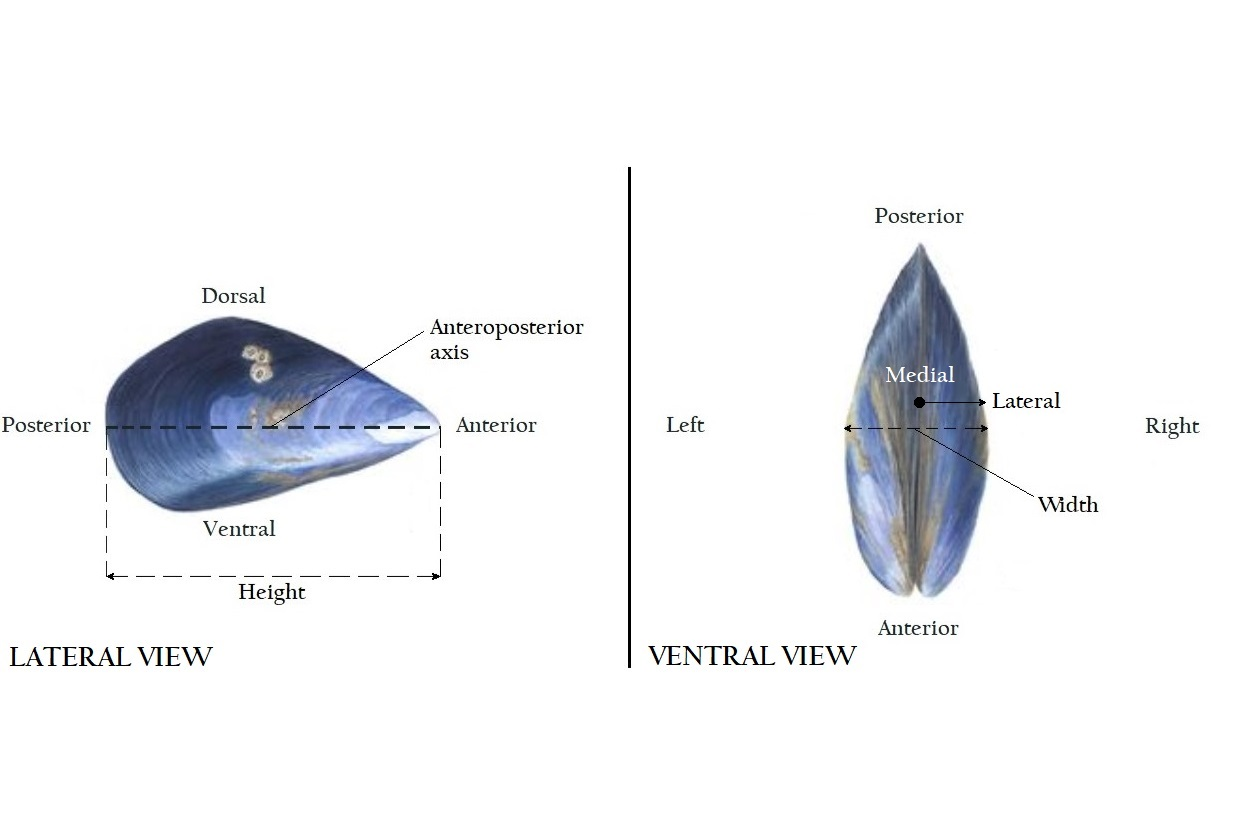
\includegraphics[width=\textwidth]{figures/Anatomy/M_edulis_anatomical_axis_lateral.jpg}
    \caption{The figure caption depends on if it ends up here, or in the material and method. Write when decided. The illustration was adapted from an artistic work by Abby Towne, A. Towne Design with permission.}
    \label{fig:anatomical_axis}
\end{figure}

\begin{table}[H]
	\centering
	\caption{Information that should be included on a score sheet for the mussel micronucleus cytome assay (in: \cite{Bolognesi2012}).}
	\label{tb:MN_Scoring}
	\begin{tabular}{ll}
		\midrule
1  &  Total number of cells scored (for differential count) \\
2  &  The number of granular and agranular cells per 1,000 \\
3  &  Number of cells scored (>1,000 agranular cells) \\
4  &  Number of necrotic cells \\
5  &  Number of apoptotic cells \\
6  &  Number of micronucleated cells \\
7  &  Total number of micronuclei and per 1,000 \\
8  &  Number of nuclear buds \\
		\bottomrule
	\end{tabular}
\end{table}

\section{Bivalve molluscs}






\section{Classification of the haemocyte subpopulations of \emph{M. edulis}}
\label{subsection:haemocyte_classification}
Since the first written account on the subject (\cite{Cuenot1891}, cited in: \cite{Cheng1980}), several authors have devoted their attentions to developing a unifying classification system for the amoebocytic blood cells of bivalve mollusks, more commonly known as haemocytes (\cite{Cheng1980, delaBallina2022}). Belonging to the bivalve familiy \emph{Mytilidae}, the haemocytes of \emph{Mytilus edulis}, \emph{Mytilus galloprovincialis} and several other commercially important species of the genus \emph{Mytilus} have been encompassed by these efforts, creating a substantial pool of literature on the haemocytes of this genus alone. Despite a lack of consensus for any unifying classification system for the haemocytes of this phylum at large, the literature that exists on the haemocytes of \emph{M. edulis} generally agrees on the existence of three distinct subpopulations.

The first effort to classify the haemocytes of \emph{M. edulis} was made by Moore and Lowe (1977). Much like the other attempts to classify bivalve haemocytes at the time, this classification was based on the morphofunctional aspects of these cells - a system that has been extensively reviewed by Hine (1999). Moore and Lowe constructed a simple classification based on static morphological and ultrastructural characteristics of the haemocytes, combined with their phagocytic capacities (\cite{Moore1977}). From routine cytological staining, they identified three haemocyte subpopulations (or cell types): "(1) small basophilic hyaline cells or lymphocytes, (2) larger basophilic hemocytes with varying degrees of irregular cytoplasmic granulation and vacuolation, and (3) eosinophilic granular haemocytes or granulocytes" (\cite{Moore1977}). The small basophilic cells (4-6 \micro m) were generally spherical in outline, had a scant thin rim of basophilic hyaline (read: transparent) cytoplasm and a spherical nucleus - bearing resemblance to vertebrate lymphocytes. The larger granular basophils (7-10 \micro m) displayed less intense basophilic cytoplasm, lower nuclear:cytoplasmic (N:C) ratios and more irregularly shaped nuclei. The eosinophilic granulocytes were the largest cell type identified (7-12 \micro m). They had a regular spherical appearance, further characterized by a small round nucleus, low N:C ratio, and a cytoplasm filled with spherical eosinophilic granules (0.5-1.0 \micro m).

Electron micrographs confirmed the existence of three ultrastructurally distinct morphologies. Except for a few mitochondria, the lymphocyte-like cells contained a scarcity of organelles and granules. This stood in sharp contrast to the larger granular basophils, which contained Golgi apparatus, phagosomes and smaller granular inclusions - possibly representing primary lysosomes. A phagocytosis assay with experimentally injected carbon particles revealed that both granular cell types displayed phagocytic properties, while the small lymphocyte-like cells did not show any evidence for this capacity (\cite{Moore1977}).

The morphological and ultrastructural findings of Moore and Lowe (1977) have since been confirmed by several investigators (\cite{Rasmussen1985, Renwartz1990, Pipe1990, Noel1994, Pipe1997, Wootton2003}). From their stand-alone electron microscopical examinations, Pipe and colleagues (1990) made a distinction between granular haemocytes with small (0.2-0.3 \micro m) and large (0.5-1.5 \micro m) granules. By relating the two ultrastructural phenotypes to their cytological staining properties, investigators soon demonstrated that the two cell types corresponded to the basophilic and eosinophilic granular haemocytes of Moore and Lowe (\cite{Pipe1990, Noel1994}). Thus, if reduced to it's static morphological criteria, Moore and Lowe's classification of \emph{M. edulis} haemocytes coincides with the original system of Cúenot (1891). This system generally recognized three types of haemocytes in bivalves: "(1) finely granular haemocytes, (2) coarsely granular haemocytes and (3) cells with very little cytoplasm surrounding the nucleus" (\cite{Cheng1984}). 

Leaning towards a phylum-wide two-categorical classification (hyalinocytes and granulocytes), Cheng (1981) argued that a distinction between the basophillic and eosinophilic granulocytes of \emph{M. edulis} was artificial, as he saw them as being immature and mature stages of the same cell type (granulocytes), respectively. From observations of what resembled intermediate stages between the lymphocyte-like and larger basophilic cells, Moore and Lowe (1977) had argued that the basophilic cells constituted an ontogenic developmental series, with the larger phagocytic macrophages representing the final stage of maturation. This was further supported by observations of lymphocyte-like cells with mitotic figures, suggesting that it could be the stem cell of this lineage (\cite{Moore1977}). Since a few smaller eosinophilic granulocytes (5-7 \micro m) were observed in their sections, the eosinophilic granulocytes were believed to represent a distinct growth series.

This theory, as pointed out by Cheng (1984), was primarily formulated through interpretive evaluations of morphological findings, rather than being based on direct ontogenic evidence. The classification of bivalve haemocytes should ideally be constructed on the basis of their ontogeny. However, mapping of ontogenic lineages among bivalve haemocytes have been tempered by the lack availible molecular databases, no one unifying model species, combined with uncertainty regarding the hematompoietic tissue(s) and processes of bivalves (\cite{Hine1999, Smith2016, Pila2016, delaBallina2022}). With no real ontogenic evidence to work with, a careful assessment of availible morphological data may represent a better alternative relative to a classification based solely on biochemistry and function (\cite{Hine1999}). 

\subsection{Flow cytometric classification of \emph{M. edulis} haemocytes}
Almost two decades after flow cytometers became commercially availible in the 1970s (\cite{Shapiro2004}), the application of these instruments started to gain traction within the field of invertebrate immunopathology (\cite{Fisher1988}). Since the traditional characterization of bivalve haemocytes were largely based on morphological criteria such as size, granularity and staining affinities, the simultaneous measurement of forward scatter (\acrshort{fsc}, $\approx$ size) and side scatter (\acrshort{ssc}, internal complexity $\approx$ granularity) represented a far less subjective approach to their characterization (\cite{AshtonAlcox1998, Allam2002, Mateo2009}).

A detailed flow cytometric characterization of the haemocytes of \emph{M. edulis} was undertaken by Le Foll and colleagues (2010), who were able to distinguish three subpopulations according to their cell diameters (\micro m) and Side Scatter (\acrshort{ssc}) (\cite{LeFoll2010}). These comprised one population of small cells (7.14$\pm{0.05}$ \micro m) with low \acrshort{ssc}, one population of larger cells (9.97$\pm{0.17}$ \micro m) with intermediate \acrshort{ssc} and one population of large cells (10.08$\pm{0.24}$ \micro m) with high \acrshort{ssc}. By running haemocytes stained with eosin - which is fluorescent in the green/yellow spectrum under blue laser exitation (\cite{Elfer2016, Koegle2020}) - their results suggested that the latter cluster to corresponded to the eosinophilic granulocytes. However, these results were not visually verified by microscopy. The use of flow cytometers equipped with cell sorting capabilities simplifies the process of verifying any classification derived from flow cytometric measurements (\cite{Shapiro2004}). However, when extracting cells with known measured characteristics is not possible, the cells to be classified can be separated by other means prior to flow cytometric acquisition.

Since the three haemocyte cell types of \emph{M. edulis} differ with regard to the size and density of their granules, Friebel (1995) and Pipe (1997) managed to physically separate the eosinophilic granulocytes from the two basophilic cell types by isopycnic centrifugation (\cite{Friebel1995, Pipe1997}). Depending on the fixative used, the whole haemocyte population separated into three or four distinct cell-bands in the interfaces of the various layers. The two basophillic cell types could be isolated in high purity from the upper cell band (lowest density), the eosinophilic granulocytes from the lower, while the intermediate fractions often consisted of varying proportions of all three cell types. Accompanied by the rapid growth of flow cytometric applications in invertebrate immunology, the progress made by Friebel (1995) and Pipe (1997) meant that results from functional and biochemical assays could be assigned to specific cell types at a higher throughput. Thus, the unraveling of the roles of individual haemocyte subpopulations really started to pick up speed.

\subsection{The role of haemocytes}
Present the difference in phagocytic capacity between the three cell types (include different types of materials).
Cytochemistry, enzyme content and cytotoxic secreted molecules in host defence, Surface receptors.
Ultrastructural findings: what organelles are found in the different cell types, and what they suggest about function.
The  eosinophilic granular cells in  M. edulis are the most active in phagocytosis and superoxide production (Pipe  et al., 1997)


\subsubsection{Scoring of micronuclei and nuclear buds}
The protocol proposed scoring of MNi in agranular haemocytes, which were characterized by their small size (3-4 \micro m), high N:C ratio and lack or low abundance of cytoplasmic granules and organelles (\cite{Bolognesi2012}). This suggestion was based on the findings of Vernier et al. (1997), who reported that the eosinophilic granulocytes of \emph{M. galloprovincialis} were less sensitive to MN induction by Benzo[a]pyrene. However, Vernier and colleagues were not able to establish wether their "agranular haemocytes" corresponded to basophilic granulocytes or non-lymphocyte-like agranular cells in the original publication, but later referred to them as hyalinocytes in the work cited by Bolognesi and Fenech (2012) (\cite{Dolcetti2002}). The attached photomicrographs of micronucleated agranular haemocytes did however represent large basophilic haemocyte with cytoplasmic vacuolation (\cite{Venier1997, Dolcetti2002}), i.e., not the small agranular haemocyte (3-4 \micro m) of Bolognesi and Fenech (2012). This celltype has been characterized as granulocytes with small granules in \emph{M. galloprovincialis} (\cite{Carballal1997}), which are equivalent to the larger granular basophils of \emph{M. edulis} (\cite{Moore1977}).

While there are discrepancies between the proposed target cell and the underlying argumentation by Bolognesi and Fenech (2012), the proposition may still be sound in context of micronucleus formation and the current scientific understanding of bivalve hematopoiesis. The "agranular haemocytes" of Bolognesi and Fenech have many names (small hyaline, blast-like, lymphocyte-like, hemoblast-like cells, etc.), but they are all invariably describing small agranular cells with very little cytoplasm surrounding the nucleus. Since their basophilia indicates the presence of free ribosomes and immaturity, while their lack of cytoplasmic organelles precludes a secretory or phagocytic function, these cells are thought to represent the immature "prohemocyte" precursor of one or both granular cell types (\cite{Hine1999, delaBallina2022, Smith2016}). The eosinophilic granulocytes have on the other hand been suggested to represent the terminal stage of differentiation in both granular cell types of \emph{Mytilus sp.} (\cite{Cheng1984}). As MNi only arise in dividing cells, this likely explains why Vernier et al. (1997) found the eosinophilic granulocytes to be less sensitive targets of cytogenic damage.

However, scoring MNi in small agranular cells exclusively may be unattainable (or just very time-consuming) in certain individuals, considering that the small agranular haemocytes of \emph{M. edulis} ($\leq$ 6 \micro m) can make up as little as 2\% of the total haemocyte population (present work). Moreover, as their nucleus is only surrounded by thin rim of cytoplasm, there is frequently insufficient space for the micronuclear boundary to be distinguishable from the main nucleus. This particular attribute complicates the process of discerning between MNi vs. NBUDs in small agranular haemocytes. Scoring of MNi in \emph{Mytilus sp.} should therefore be broadened to include all basophilic or "hyaline" cells.

